The \gls{id} is designed to provide good track reconstruction, precise momentum
resolution and both primary and secondary vertex measurements (see
Section~\ref{sec:primary-vertex}) above a nominal $\pt$ threshold of 0.5~GeV and
within the pseudorapidity $|\eta| < 2.5$. It also provides electron
identification over $|\eta| < 2.0$ for energies between 0.5~GeV and
150~GeV~\cite{ATLASPaper}. The ID is 6.2~m long and has a radius of about 1.1~m,
it is surrounded by a solenoidal magnetic field of 2~T. Its layout is
schematized in Figure~\ref{fig:id} and, as can be seen, it is composed of three
sub-detectors.

At the inner radius the \emph{pixel detector} mostly determines the position of
primary and secondary vertex. The silicon sensors are 250~$\mu$m thick detectors
that operate with an initial bias voltage of $\sim$150~V that, due to the high
radiation level, will increase up to 600~V after 10 years of operation to
maintain a good charge collection.

In the middle layer of the ID the \gls{sct} is designed to give eight precision
measurements per track which contributes to determine the primary and secondary
vertex position and momentum measurements. The silicon sensors are 285
$\pm 15 \mu$m thick and initially operates with a bias voltage of $\sim$150~V
which will increase up to 350~V after ten years of operation for good charge
collection.

The last layer of the ID is the \gls{trt}, it contributes to tracking and
identification of charged particles. It consists of drift (straw) tubes, 4~mm in
diameter with a 31~$\mu$m wire in the center of each straw, filled with a gas
mixture of 70\% Xe, 27\% CO$_2$ and 3\% O$_2$. These tubes substantially act
like proportional counters where the tube is the cathode and kept at $- 1.5$~kV
and the wire is the anode and grounded. When a charged particle cross one tube,
leaves a signal; the set of signals in the tubes, reconstructs to a track which
represents the path of the crossing object. The space between the straw tubes is
filled with material with different refraction index, this causes charged
particles crossing it to emit transition radiation thus leading to some straw to
have a much stronger signal. The transition radiation depends on the speed of
the particles which in turn depends on the initial energy and the mass of the
particles thus lighter particles will have higher transition energy and stronger
signal in the straw tubes. Tracks with several strong signal straw, can be
identified as belonging to electrons (the lightest charged particle).

An additional layer, the \gls{ibl}, was recently added in the region between the
beam pipe and the inner pixel layer (B-layer). It is designed to increase the
tracking robustness by replacing damaged parts of the pixel B-layer and
increasing the hit redundancy with the higher luminosity (twice the design
luminosity) foreseen for the \gls{hl-lhc} in 2020, moreover, being closer to the
beam pipe it increases the impact parameter measurement precision. As part of
the installation procedure a smaller beam pipe was installed which will be used
also in the HL-LHC phase unless an even smaller radius pipe becomes
possible~\cite{IBL}.

\begin{figure}[!h]
  \centering
    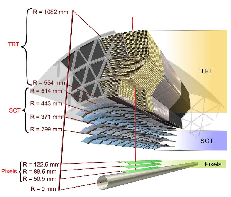
\includegraphics[width=.5\linewidth]{inner_detector}
    \caption{Schematic view of a charged track of 10~GeV $\pt$ that traverses
      the different ID sub-detectors. After traversing the beryllium pipe, the
      track passes through the three cylindrical silicon-pixel layers, the four
      layers of silicon-microstrip sensors (SCT) and the approximately 36 straws
      contained in the TRT within their support structure.}
    \label{fig:id}
\end{figure}
%%% Local Variables:
%%% mode: latex
%%% TeX-master: "../search_for_DM_LED_with_ATLAS"
%%% End:
